\chapter{Background}\label{chapter:background}

This chapter presents an overview of \Beluga, and \Harpoon, whose implementations were modified as part of this thesis.
Topics in the design of a programming language's concrete syntax are discussed, along with features found in parsers of languages for proof assistants.
Then, the concept of incremental proof and program development is briefly explained to motivate those modifications.
Finally, the design and implementation of incremental development is examined for various proof assistants.

\section{The \Beluga Language}

In \Beluga, theorems are encoded using contextual \LF, its index language, and proofs are encoded as programs.
Logic propositions are represented as \LF type families with term-level constants parameterized by $\beta$-normal $\eta$-long \LF terms to construct witnesses for these propositions~\cite{nanevski2008contextual, foundation2008pientka, DBLP:journals/corr/abs-1009-2789}.
To facilitate the implementation of semantic analysis, and because \LF kinds, types and terms are strongly normalizing~\cite{harper1993framework}, they are required to be encoded in normal form by the user.
\Beluga extends \LF to support explicit contexts and substitutions, which enables mechanized reasoning with respect to assumptions, like in proofs on paper~\cite{pientka2010programming}.
This means that terms containing free variables can be manipulated and reasoned about explicitly.

To illustrate how \Beluga is leveraged to mechanically prove properties about formal systems, consider the following example adapted from \cite{felty2010reasoning} where it is shown that algorithmic equality for an untyped $\lambda$-calculus is reflexive.
The abstract syntax for this calculus is first defined in figure~\ref{figure:running-example-abstract-syntax}, which is encoded as an \LF type constant \verb|term| with term constants \verb|lam|, \verb|app| and \verb|unit| in the \verb|Term| module of figure~\ref{figure:running-example-implementation}.
Then, the algorithmic equality judgment for terms is defined in figure~\ref{figure:running-example-equality} and encoded as an \LF type family \verb|≡|, using an infix notation, in module \verb|Algorithmic_equality|.
Note that this definition for equality does not provide constants to construct witnesses of reflexivity, symmetry or transitivity.
These properties may instead be derived, like theorem~\ref{theorem:reflexivity} for reflexivity.
This corresponds to the \verb|refl| recursive program of figure~\ref{figure:running-example-implementation} which constructively shows that for any (possibly open) term $M$, the algorithmic equality $M \equiv M$ holds.
The notion that $M$ may contain free variables comes into play when proving reflexivity for terms of the form $\lambda x. M$ since the induction hypothesis requires assumptions about the function parameter $x$.

\begin{figure}[H]
\begin{subfigure}{\linewidth}
\centering
\begin{tabular}{p{2cm} >{\raggedleft}p{1cm} r l}
Terms & $M, N$ & $\Coloneqq$ & $x \mid \lambda x. M \mid M\ N \mid \Unit$
\end{tabular}
\caption{%
Syntax definition for the untyped $\lambda$-calculus used in the running example.
}
\label{figure:running-example-abstract-syntax}
\end{subfigure}
\par\bigskip
\begin{subfigure}{\linewidth}
{\footnotesize
\begin{mdframed}[frametitle={$\boxed{\Gamma \vdash M \equiv N}$ : the term $M$ is algorithmically equal to $N$ in context $\Gamma$}]
\begin{equation}
\infer[\equiv\text{-lam}]{\Gamma \vdash \lambda x. M \equiv \lambda x. N}{\Gamma, x : \mathsf{term}, e : x \equiv x \vdash M\ x \equiv N\ x}
\end{equation}
\begin{equation}
\infer[\equiv\text{-app}]{\Gamma \vdash M_1\ M_2 \equiv N_1\ N_2}{\Gamma \vdash M_1 \equiv N_1 & \Gamma \vdash M_2 \equiv N_2}
\end{equation}
\begin{equation}
\infer[\equiv\text{-unit}]{\Gamma \vdash \Unit \equiv \Unit}{}
\end{equation}
\end{mdframed}
}
\caption{Definition of algorithmic equality for terms in this $\lambda$-calculus.}
\end{subfigure}
\caption[Running example of algorithmic equality for an untyped $\lambda$-calculus]{%
Running example.
}
\label{figure:running-example-equality}
\end{figure}%
\begin{figure}\ContinuedFloat
\begin{subfigure}{\linewidth}
\begin{theorem}
\label{theorem:reflexivity}
If $\Gamma$ is a context where $(x : \mathsf{term}) \in \Gamma$ is sufficient for $(e : x \equiv x) \in \Gamma$, and $\deduce{\Gamma \vdash \Term{M}}{\D}$, then $\Gamma \vdash M \equiv M$.
\end{theorem}
{\footnotesize
\begin{proof}
By structural induction on $\D$:
\begin{itemize}
\item
Case $\D = \infer[\text{term-var}]{\Gamma \vdash \Term{x}}{\deduce{(x : \mathsf{term}) \in \Gamma}{\D'}}$.
\par
By the regular context specification on $ \D' $, we have $(e : x \equiv x) \in \Gamma$, hence $\Gamma \vdash x \equiv x$.
\item
Case $\D = \infer[\text{term-lam}]{\Gamma \vdash \Term{\lambda x. N}}{\deduce{\Gamma, x : \mathsf{term} \vdash \Term{N}}{\D'}}$.
\par
By weakening on $\D'$, we have $\deduce{\Gamma, x : \mathsf{term}, e : x \equiv x \vdash \Term{N}}{\E}$.
\par
By the induction hypothesis on $\E$, we have $\deduce{\Gamma, x : \mathsf{term}, e : x \equiv x \vdash N\ x \equiv N\ x}{\E'}$.
\par
Then,
\begin{equation*}
\infer[\equiv\text{-lam}]{\Gamma \vdash \lambda x. N \equiv \lambda x. N}{\deduce{\Gamma, x : \mathsf{term}, e : x \equiv x \vdash N\ x \equiv N\ x}{\E'}}.
\end{equation*}
\item
Case $\D = \infer[\text{term-app}]{\Gamma \vdash \Term{M_1\ M_2}}{\deduce{\Gamma \vdash \Term{M_1}}{\D_1} & \deduce{\Gamma \vdash \Term{M_2}}{\D_2}}$.
\par
By the induction hypothesis on $\D_1$, we have $\deduce{\Gamma \vdash M_1 \equiv M_1}{\E_1}$.
\par
By the induction hypothesis on $\D_2$, we have $\deduce{\Gamma \vdash M_2 \equiv M_2}{\E_2}$.
\par
Then,
\begin{equation*}
\infer[\equiv\text{-app}]{\Gamma \vdash M_1\ M_2 \equiv M_1\ M_2}{\deduce{\Gamma \vdash M_1 \equiv M_1}{\E_1} & \deduce{\Gamma \vdash M_2 \equiv M_2}{\E_2}}.
\end{equation*}
\item
Case $\D = \infer[\text{term-unit}]{\Gamma \vdash \Term{\Unit}}{}$.
\par
This case holds by $\equiv\text{-unit}$.
\end{itemize}
\end{proof}
}
\caption{On paper proof of algorithmic equality for this $\lambda$-calculus.}
\end{subfigure}
\caption[]{Running example (contd.).}
\end{figure}%
\begin{figure}\ContinuedFloat
\begin{subfigure}{\linewidth}
\begin{Verbatim}[commandchars=\\\{\}, baselinestretch=1, numbers=left]
\verbbf{module} Term = \verbbf{struct}
  \verbbf{LF} term : \verbbf{type} =
  | lam : (term \makebox[1em]{→} term) \makebox[1em]{→} term
  | app : term \makebox[1em]{→} term \makebox[1em]{→} term
  | unit : term;
  \verbprag{--name term M.}
\verbbf{end}

\verbbf{module} Algorithmic_equality = \verbbf{struct}
  \verbprag{--open Term.}
  \verbprag{--infix \makebox[1em]{≡} none.}
  \verbbf{LF} \makebox[1em]{≡} : term \makebox[1em]{→} term \makebox[1em]{→} \verbbf{type} =
  | lam : (\{x : term\} \makebox[1em]{→} x \makebox[1em]{≡} x \makebox[1em]{→} M x \makebox[1em]{≡} N x) \makebox[1em]{→} Term.lam M \makebox[1em]{≡} Term.lam N
  | app : M1 \makebox[1em]{≡} N1 \makebox[1em]{→} M2 \makebox[1em]{≡} N2 \makebox[1em]{→} Term.app M1 M2 \makebox[1em]{≡} Term.app N1 N2
  | unit : Term.unit \makebox[1em]{≡} Term.unit;
\verbbf{end}

\verbprag{--open Term.}
\verbprag{--open Algorithmic_equality.}

\verbbf{schema} ctx = \verbbf{block} (x : term, eq : x \makebox[1em]{≡} x);

\verbbf{rec} refl : (g : ctx) \makebox[1em]{→} \{M : [g \makebox[1em]{⊢} term]\} \makebox[1em]{→} [g \makebox[1em]{⊢} M \makebox[1em]{≡} M] =
  / total d (refl _ d) /
  \verbbf{mlam} M \makebox[1em]{⇒}
    \verbbf{case} [_ \makebox[1em]{⊢} M] \verbbf{of}
    | [g \makebox[1em]{⊢} #p.x] \makebox[1em]{⇒} [g \makebox[1em]{⊢} #p.eq]
    | [g \makebox[1em]{⊢} Term.lam {\textbackslash}x. F] \makebox[1em]{⇒}
        \verbbf{let} [g, b : \verbbf{block} (x : term, eq : x \makebox[1em]{≡} x) \makebox[1em]{⊢} D] =
          refl [g, b : \verbbf{block} (x : term, eq : x \makebox[1em]{≡} x) \makebox[1em]{⊢} F[\monoellipsis, b.x]]
        \verbbf{in}
        [g \makebox[1em]{⊢} Algorithmic_equality.lam {\textbackslash}x. {\textbackslash}eq. D[\monoellipsis, <x; eq>]]
    | [g \makebox[1em]{⊢} Term.app M1 M2] \makebox[1em]{⇒}
        \verbbf{let} [g \makebox[1em]{⊢} D1] = refl [g \makebox[1em]{⊢} M1] \verbbf{in}
        \verbbf{let} [g \makebox[1em]{⊢} D2] = refl [g \makebox[1em]{⊢} M2] \verbbf{in}
        [g \makebox[1em]{⊢} Algorithmic_equality.app D1 D2]
    | [g \makebox[1em]{⊢} Term.unit] \makebox[1em]{⇒} [g \makebox[1em]{⊢} Algorithmic_equality.unit];
\end{Verbatim}
\caption[Algorithmic equality in \Beluga]{%
Mechanized proof of algorithmic equality in \Beluga for this $\lambda$-calculus, adapted from \cite{felty2010reasoning}.
}
\label{figure:running-example-implementation}
\end{subfigure}
\caption[]{Running example (contd.).}
\label{figure:running-example}
\end{figure}

\clearpage

As illustrated in figure~\ref{figure:running-example-implementation}, a signature in \Beluga is the list of all the toplevel constant declarations in a mechanization.
This includes the aforementioned \LF type-level and term-level constant declarations, but also includes inductive and coinductive type declarations at the computation-level, with their associated constructors and destructors respectively, and computation-level programs.
Modules can be declared as well to introduce namespaces, which allows constant names to be reused and offers a way of organizing mechanizations.
Though it is not showcased in that example, \Harpoon provides an alternative to specifying proofs as programs in the form of a proof script comprised of tactics and their effects on the meta-level and computation-level contexts for variables.
A complete specification of the concrete syntax for signature-level declarations is provided in section~\ref{section:syntax-signature} as part of grammars for parsing.
To discuss the statics and dynamics of \Beluga, an abstract syntax definition like the following is used instead.

Let $x$ and $c$ range over computation-level variables and constants respectively, $X$ range over meta-object variables, $\psi$ over context variables and $g$ over context schemas.
Figure~\ref{figure:internal-syntax} then provides an overview of \Beluga's core language.
\LF kinds classify \LF types, which classify \LF terms.
Likewise, computation-level kinds classify computation-level types, which classify computation-level expressions.
\LF terms are broken down into normal and neutral terms, along with heads and spines, to syntactically enforce canonical forms.
The notation $A \to K$ is used for the \LF kind $\Pi x{:}A. K$ when $x$ does not appear free in $K$.
The notation $A \to B$ is defined analogously for \LF types.
Since \Beluga's type system is bidirectional, the syntax of computation-level expressions is split into those for which a type can be inferred (type-synthesizing expressions), and those that can be checked against a type (type-checkable expressions).
Meta-objects, classified by meta-types, can be embedded in the computation-level by way of boxes that simultaneously bind all variables from \LF contexts.
Pattern-matching over type-synthesizing expressions (which includes embedded meta-objects) is supported by way of patterns, whose abstract syntax is omitted from figure~\ref{figure:internal-syntax} for the sake of conciseness.

\begin{figure}
\begin{subfigure}{\linewidth}
\begin{tabular}{p{5.5cm} >{\raggedleft}p{1cm} r l}
\LF kinds & $K$ & $\Coloneqq$ & $\Pi x{:}A. K \mid \mathbf{type}$\\
\LF types & $A, B$ & $\Coloneqq$ & $\Pi x{:}A. B \mid P$\\
Atomic \LF types & $P$ & $\Coloneqq$ & $a\ S$\\
\LF normal terms & $M$ & $\Coloneqq$ & $R \mid \lambda x. M$\\
\LF neutral terms & $R$ & $\Coloneqq$ & $H\ S \mid u[\sigma]$\\
\LF heads & $H$ & $\Coloneqq$ & $x \mid c \mid p[\sigma]$\\
\LF spines & $S$ & $\Coloneqq$ & $\cdot \mid M\ S$\\
Substitutions & $\sigma$ & $\Coloneqq$ & $\cdot \mid \mathsf{id}_\psi \mid \sigma, M \mid \mathsf{id}_\psi[\rho]$\\
Substitution closures & $\rho$ & $\Coloneqq$ & $s[\sigma]$\\
Contexts & $\Psi$ & $\Coloneqq$ & $\cdot \mid \psi \mid \Psi, x : A$\\
\end{tabular}
\caption{Internal syntax of contextual \LF in \Beluga.}
\end{subfigure}
\par\bigskip
\begin{subfigure}{\linewidth}
\begin{tabular}{p{5.5cm} >{\raggedleft}p{1cm} r l}
Meta-types & $U$ & $\Coloneqq$ & $\cdots \mid g \mid (\Psi \vdash A) \mid (\Psi \vdash \Psi)$\\
Meta-objects & $C$ & $\Coloneqq$ & $\cdots \mid \Psi \mid (\Psi \vdash M) \mid (\Psi \vdash \sigma)$
\end{tabular}
\caption{Internal syntax of \Beluga's meta level (excerpt).}
\end{subfigure}
\par\bigskip
\begin{subfigure}{\linewidth}
\begin{tabular}{p{5.5cm} >{\raggedleft}p{1cm} r l}
Computation-level kinds & $\kappa$ & $\Coloneqq$ & $[U] \to \kappa \mid \Pi X{:}U. \kappa \mid \mathbf{ctype}$\\
Computation-level types & $\tau$ & $\Coloneqq$ & $\cdots \mid c \mid \tau_1 \to \tau_2 \mid \Pi X{:}U. \tau \mid [U] \mid \tau\ [C]$\\
Type-checkable expressions & $e$ & $\Coloneqq$ & $\cdots \mid i \mid [C] \mid \mathbf{fn}\ x \Rightarrow e \mid \mathbf{mlam}\ X \Rightarrow e$ \\
& & $|$ & $\mathbf{let}\ x = i\ \mathbf{in}\ e \mid \mathbf{case}\ i\ \mathbf{of}\ \overrightarrow{p \Rightarrow e}$\\
Type-synthesizing expressions & $i$ & $\Coloneqq$ & $\cdots \mid x \mid c \mid i \ e \mid e : \tau$
\end{tabular}
\caption{Internal syntax of \Beluga's computation level (excerpt).}
\end{subfigure}
\caption[Excerpt of \Beluga's internal syntax]{%
Excerpt of \Beluga's internal syntax~\cite{nanevski2008contextual, germain2010implementation, cave2013first, ferreira2013compiling} used in discussions about its theory.
}
\label{figure:internal-syntax}
\end{figure}

\section{The Legacy Implementation of \Beluga} \label{section:beluga-implementation}

This section presents an overview of the implementation of \Beluga before any contribution detailed in this thesis were made\footnote{The implementation of \Beluga at revision hash \href{https://github.com/Beluga-lang/Beluga/tree/3db1ffd08d4c3bde7ad2ceb924bfb95488eef2b2}{3db1ffd08d4c3bde7ad2ceb924bfb95488eef2b2, available on GitHub.}}.
This initial description serves as the basis for all performance and design comparisons made with respect to \Beluga version~\texttt{1.1}.

\Beluga is implemented following the pipeline architectural pattern, whereby processing of a signature is implemented in distinct phases, and data flows in a feed-forward fashion throughout.
The compilation of \Beluga programs to machine code is not supported, so the implementation only covers the frontend component of compilation, which is responsible for syntactic and semantic analysis of programs.
Since \Beluga is a dependently-typed language featuring code coverage analysis and termination checking, this semantic analysis process is complex.

\begin{figure}
\centering
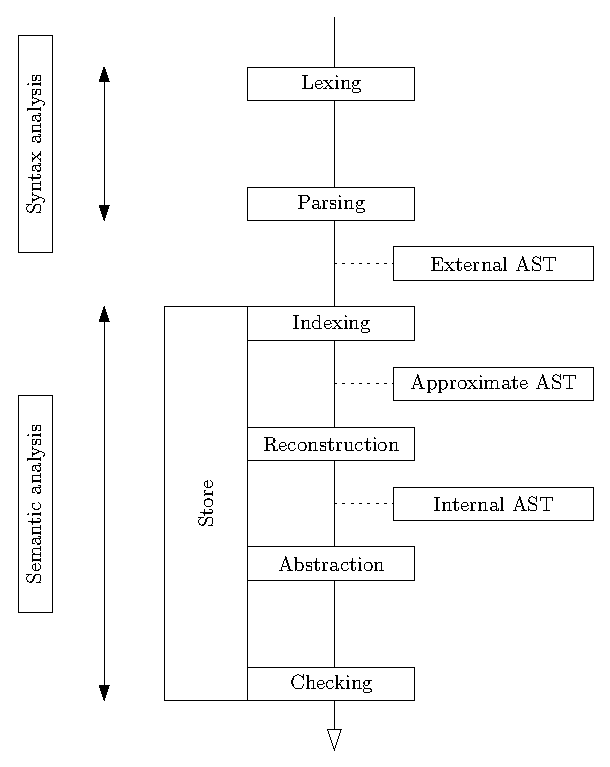
\includegraphics{figures/legacy-beluga-processing-pipeline.eps}
\caption[Overview of \Beluga version \texttt{1.0}'s processing pipeline]{%
Overview of the implementation of \Beluga version \texttt{1.0}'s processing pipeline.
The syntax analysis process converts the textual representation of \Beluga programs into an initial \acs{AST}.
The semantic analysis process refines this \acs{AST} by performing type-directed signature reconstruction using global mutable data structures.
This includes a store of constant declarations in the signature, along with auxiliary data for name resolution, fresh name generation and relations between type families.
}
\label{figure:legacy-beluga-processing-pipeline}
\end{figure}

As illustrated in figure~\ref{figure:legacy-beluga-processing-pipeline}, the processing of a \Beluga signature starts with syntax analysis, which is comprised of a tokenization and parsing phase that converts the textual representation of the signature to an \ac{AST}, called the external \ac{AST}.
The model for this \ac{AST} contains ambiguous nodes, meaning that some \ac{AST} node variants capture multiple parse trees.
Specifically, the application of \LF type-level and term-level constants is represented as a list of parsemes, which effectively postpones the parsing of applications featuring user-defined operator notations.
Parsing of signature-level declarations also features auxiliary data and routines for mixing or unmixing parsemes to delegate some disambiguation to phases after context-free parsing.

Indexing in \Beluga is the process by which the concrete syntax is elaborated to a locally nameless representation called the approximate syntax, wherein bound variables are replaced with their corresponding de Bruijn indices, and constant names are replaced with symbolic identifiers defined in the centralized store of declarations.
For instance, the \LF term $\lambda x. \lambda y. \lambda z.\ x\ z\ (y\ z)$ is indexed as $\lambda\ \lambda\ \lambda\ 3\ 1\ (2\ 1)$.
As part of \Beluga's design for terse type declarations and programs, some terms may contain free variables, like the variables \verb|M1|, \verb|M2|, \verb|N1| and \verb|N2| in the definition of constant \verb|Algorithmic_equality.app| in figure~\ref{figure:running-example-implementation}.
The computation of de Bruijn indices of those free variables is postponed until the abstraction phase.
Indexing is run immediately after parsing, and is additionally responsible for disambiguating the juxtaposition of \LF parsemes at the precedence level of applications (which may contain user-defined operators), as well as disambiguating \LF types from terms and resolving constants.
This design is sensible since computing de Bruijn indices requires a stateful traversal of the \ac{AST} that accumulates lists of bindings to produce the referencing environment.
Using the store, some measure of identifier overloading is supported using a pre-defined order of lookups in the referencing environment based on the kind of identifier that is expected for a given \ac{AST} node.
For instance, computation-level identifiers are resolved by looking up in order the store of computation-level variables, the store of program constants, and then the store of data type constructors.
Since names appearing in the \LF level are not part of this name resolution strategy, then an identifier can be overloaded to stand for an \LF term as well as a computation-level expression.

After indexing, the reconstruction~\cite{pientka2013insider} phase is run to reconstruct holes in types and terms, both at the \LF level and the computation level.
These holes stand for arguments omitted by the user, and provide an elegant way of abbreviating otherwise tedious aspects of programming with dependent types.
For instance, in the \verb|refl| program of figure~\ref{figure:running-example-implementation}, the context parameter \verb|(g : ctx)| is implicit, meaning that calls like \verb|refl m| actually denote \verb|refl _ m|, with a hole \verb|_| where a context argument is expected.
This is admissible because any argument for that parameter can be reconstructed from the argument \verb|m| given for the explicit parameter \verb|{M : [g ⊢ term]}|, which is defined with respect to \verb|g|.
At the \LF level, approximate types are constructed to partially check the kinding of \LF types and the typing of \LF terms, as well as for guiding the synthesis of normal terms that check against a given type using typing constraints.
Type-driven unmixing of overloaded syntactic forms occurs at the meta-level, whereby meta-objects are disambiguated from substitutions during reconstruction.
The approximate \ac{AST} provides a disambiguated representation of the overall \Beluga signatures, which helps in keeping track of the various changes made during this complicated phase.

A nearly complete internal \ac{AST} as defined in figure~\ref{figure:internal-syntax} is produced at the end of reconstruction.
An abstraction phase~\cite{germain2010implementation} is run to abstract over free variables, which effectively introduces binders for implicit parameters, and unrolls the contexts of variables used during type-driven reconstruction.
For instance, the \LF term constant \verb|Algorithmic_equality.app| of figure~\ref{figure:running-example-implementation} is abstracted to

\bigskip
\begin{Verbatim}[commandchars=\\\{\}, baselinestretch=1]
(M1 : term) → (N1 : term) → (M2 : term) → (N2 : term) →
  (_ : M1 \makebox[1em]{≡} N1) \makebox[1em]{→} (_ : M2 \makebox[1em]{≡} N2) \makebox[1em]{→} Term.app M1 M2 \makebox[1em]{≡} Term.app N1 N2
\end{Verbatim}

\noindent
and then de Bruijn indices are recomputed, which yields
\begin{equation*}
\Pi_{\texttt{term}}\ \Pi_{\texttt{term}}\ \Pi_{\texttt{term}}\ \Pi_{\texttt{term}}\ \Pi_{4 \equiv 3} \Pi_{3 \makebox[1em]{≡} 2}\ \texttt{Term.app}\ 6\ 4\ \equiv \texttt{Term.app}\ 5\ 3
\end{equation*}
This phase completes the desugaring of \Beluga programs since it finishes the computation of de Bruijn indices for variables across all levels.
The main technical challenge abstraction runs into is determining the order in which introduced binders must appear so that dependencies on terms are preserved in inferred dependent types.
This includes identifying and handling circular dependencies in abstracted parameters.

Finally, a semantic checking phase is run to ensure signature reconstruction and abstraction yielded valid programs.
This includes performing type-checking, coverage-checking and totality-checking.
These processes guarantee, respectively, that \LF-level and computation-level expressions are well-typed, that case analyses are exhaustive, and that functions annotated with a totality declaration terminate for all inputs.
Typing and coverage constraints generated during theses checking processes are statefully shared throughout this phase.
Leftover and unresolved constraints in the state after having fully processed a program unit are used to signal to the user that that program is unsound within \Beluga's system.

The flow of data in the implementation of \Beluga is complex, like in most software systems.
Starting with the indexing phase, data is shared between the phases of signature reconstruction using a global mutable store.
This auxiliary data structure is a set of tables mapping constant identifiers to metadata, like in a relational database.
Crucially, the referencing environment used during indexing is computed using this store.
At any given point during the processing pipeline, the store's state is valid since program units are processed sequentially.
New program units may be safely appended afterwards in interactive sessions.

\section{The \Harpoon Interactive Proof Environment}\label{section:harpoon-background}

The \Beluga system provides two ways to interactively perform queries on an existing \Beluga signature, or to augment it with new theorems.
These are the legacy \ac{REPL} and the \Harpoon system~\cite{errington2021harpoon}, the latter of which is designed as a replacement for the former.
Both systems allow the user to input \LF-level terms or computation-level expressions and get their type inferred with respect to an already elaborated \Beluga signature.
\Harpoon further enables the interactive definition and proving of theorems using sets of tactics aimed at automating proof development.
Both the \ac{REPL} and \Harpoon depend on the processing phases of \Beluga and the flow of information therein as described in the previous section.

\Harpoon is a structural editor for proof scripts that can be translated into \Beluga programs.
To do so, it provides edit actions a user may perform in an interactive proof session.
These actions are split into two categories, namely administrative commands and proof tactics.
\begin{itemize}
\item
Administrative commands affect the ambient state of the \ac{REPL} by allowing the user to navigate in the \Beluga signature and in the history of executed actions.
These include navigating between incomplete subgoals in a theorem, navigating to incomplete proof scripts, undoing and redoing proof tactics, renaming bound variables, and persisting the changes made to the signature.
\item
Proof tactics affect the state of the proof script under edit.
These include tactics such as \verb|intros| to universally quantify over the current theorem's premises and \verb|split| to perform a case analysis on the structure of a value.
\Harpoon also features a \verb|suffices| tactic allowing for backwards reasoning on a given subgoal, as well as tactics to perform automated proof search.
\end{itemize}

In order for \Harpoon edit actions to be sound, they must bring the structural editing session from a valid state to another valid state.
For proof tactics, this involves carefully keeping track of induction hypotheses generated during case analyses, as well as maintaining a correct record of identifiers in scope at the node under edit in the proof script.
For administrative commands, the state of identifiers in scope has to always be local to the location in the \Beluga signature where the current theorem is declared, and undoing edit actions has to restore the current proof script to its previous state.
This in particular requires that effects occurring in type-checking and unification be undoable as well, which includes being able to revert the instantiation of unification variables.

In release \texttt{v1.0} of \Beluga and \Harpoon, not all administrative commands are sound, specifically with regards to the state of identifiers in scope.
This is explored in chapter~\ref{chapter:indexing-reimplementation}, with a detailed explanation on the soundness issues and solutions to rectify them.

\section{Parsing and Programming Language Design}\label{section:background-parsing}

% What is parsing?

In compiler design, parsing is the process of converting the textual representation of a program into a hierarchical data structure~\cite{aho2007compilers, afroozeh2019practical}, which is typically called a parse tree.
When a parse tree captures all the data about the text being processed, including comments and parentheses, then it is referred to as a concrete syntax tree.
Otherwise, when parts of the data have been abstracted away, it is instead called an \ac{AST}.

% What is ambiguity in parsing?

A program's textual representation is ambiguous with respect to a predefined set of parse rules if the program can be parsed into a parse forest, which is multiple parse trees~\cite{aho2007compilers}.
By way of analogy, a sentence in a natural language is ambiguous if it can be interpreted in multiple valid ways with respect to its syntactic and grammatical rules.
Since programming languages are tools for describing computerized systems, it is necessary that each valid written program has exactly one interpretation~\cite{aho2007compilers}.
In the strictest of cases, this unicity of interpretation may be enforced at the level of the grammar and parser, such that all syntactically valid programs have exactly one inferable interpretation.
This is typically achieved using rules and syntactic conventions that prevent ambiguous programs from being ever written in the first place.

Certain kinds of syntactic ambiguities are unavoidable in programming languages, and are frequently useful to the end user.
Indeed, programming languages often reuse or overload syntactic constructs to reduce both the number and the complexity of rules that users have to learn in order to read and write programs.
Ambiguous syntax can also make programs more terse, which may improve some workflows~\cite{resolveAmbiguity}.
Additional mechanisms need to be put in place as part of the compiler's implementation to detect syntactic ambiguities, and either signal them as errors, or resolve them using additional interpretation rules.

% What is disambiguation in parsing?

Disambiguation is the process by which a parse forest is filtered down to a single parse tree.
It refers to the procedures used to resolve ambiguities in intermediate results of parsing.
In parsing systems that do not output parse forests, disambiguation typically involves manipulating the \ac{AST} representation of a single parse tree that captures ambiguities, meaning that some of its nodes represent the overlapping of syntactic constructs.
Functionally, these nodes suspend parsing until more information is available to disambiguate them to the correct node variant.

% What is the impact of disambiguation on program readability?

Increasing the amount of computation required to disambiguate the textual representation of a program negatively impacts the maintainability and readability of that program for the end user.
Indeed, some forms of ambiguity in the syntax of a program may prevent the end user from fully understanding it in isolation from the rest of the code sections.
As such, one can argue that the programmatic strategies for disambiguating the syntax of a programming language should be intuitive so that external software is not required for the end user to read a program.
For instance, name resolution is sufficiently intuitive for users, whereas searching in a parse forest for a parse tree that type-checks is not necessarily intuitive, especially given the complexity of some type systems.
Hence, trade-offs between functionality and ease of understanding must be made when designing a language.

% What are some examples of syntactic ambiguities?

Different kinds of concrete syntax ambiguities may arise during parsing of a programming language.
We distinguish three kinds of syntactic ambiguities that come into play in the implementation of \Beluga, listed below in increasing degree of cognitive complexity required to solve them:
\begin{enumerate}
\item
\textit{Static operator ambiguities}: operators and their operands may be interpreted in different orders depending on where they appear in a whitespace-delimited list of terms.
For instance, the expression $a + b * c$ is ambiguous with respect to the grammar $e\coloneqq e+e\mid e*e$.
These ambiguities are typically resolved by assigning a precedence level, a fixity and an associativity to each operator in the language, and parsing them as keywords.
\item
\textit{Name-based ambiguities}: overloaded identifiers may be resolved to different binding sites depending on where they appear in an expression, and fall under different semantic categories as a consequence.
For instance, in a dependently-typed language, type-level and term-level variables may be syntactically ambiguous, but they may have distinct syntaxes for binders.
Semantic analysis of the \ac{AST} with respect to a symbol table is usually sufficient to disambiguate those cases.
However, overloading of identifiers coupled with more advanced features, like user-defined mixfix operators~\cite{danielsson2008parsing}, poses additional challenges since identifiers may not be considered in isolation.
\item
\textit{Type-based ambiguities}: the correct interpretation of an expression may only be determined once a type has been inferred for it, or if it is checked against a type.
This does not refer to method overloading in object-oriented programming languages since the syntax for calling a method is not ambiguous.
Rather, if the expression being parsed is an identifier, then a type-based ambiguity may be that that expression or a surrounding one falls into a different syntactic category based on the identifier's type or kind.
For instance, the syntax $ \texttt{(g, x : t)} $ may denote a pair of terms, with the variable $ \texttt{x} $ being checked against the type $ \texttt{t} $, or it may denote the context $ \texttt{g} $ with an added variable declaration $ \texttt{x : t} $.
In this case, what $ \texttt{(g, x : t)} $ syntactically denotes depends on the type of $ \texttt{g} $.
To solve such ambiguities, some type information may be provided by a symbol table if the type ascribed to an identifier is known at the declaration site.
In general it is not practical to disambiguate expressions having type-based ambiguities before type-checking, especially when more intricate type inference algorithms need to be applied to determine the type of an identifier.
Because of this, languages are typically designed to avoid type-based ambiguities.
In the same way that is done in figure~\ref{figure:internal-syntax}, identifiers like $\psi$ can be reserved to always denote contexts, such that $\texttt{($\psi$, x : t)}$ is unambiguously a context.
\end{enumerate}

% What do ambiguities have to do with language design?
% What is the typical workflow for designing syntaxes and implementing parsers? What are parser generators? What are their limitations?

The kinds of syntactic ambiguities that arise in the design of a programming language depend on the system used to specify its syntax, which in turn affects the algorithm required to parse it.
The concrete syntax of programming languages is typically specified with a \ac{CFG}, denoted in \ac{EBNF}.
If a language can be specified by a \ac{CFG}, then it is a \ac{CFL}.
\Acp{CFL} have many advantages, including the fact that there is an abundance of well-vetted parser generators for such languages.
\ocamllex together with \ocamlyacc~\cite{smith2007ocamllex} is one example of such a parser generator.
Crucially, \acp{CFL} are easy to parse, both algorithmically and by the end user.
As the name suggests, parsers for \acp{CFL} do not require additional data in a context specifically intended for disambiguation.
This ensures that programs can scale and be readable by the user without having to fully know the context in which programs appear.
That is, other code sections in a \ac{CFL} do not affect how a given code section is parsed.
Static operator ambiguities as mentioned previously can be resolved by rewriting the grammar while keeping it context-free.
Name-based and type-based ambiguities however give rise to context-sensitive languages, or even strictly Turing-recognizable languages~\cite{chomsky1956three}.
Context-sensitive languages necessitate additional data about the context in which parts of a program appear to correctly parse it.
This typically means that some semantic analysis is required during parsing in order to complete the syntactic analysis.
Consequently, the concrete syntax's design for a programming language is intrinsically linked with the algorithm required to parse it.

% What are some language design considerations?

A grammar is dynamic (or user-extensible, or featuring syntax extensions) if the way a program is parsed is influenced by directives in the program itself, and otherwise the grammar is static.
Languages for specifying logics tend to favour user-extensible grammars over static ones.
Indeed, \Agda~\cite{clffolp, agda2023} and \Isabelle/\HOL~\cite{wenzel2023isabelleimpl, wenzel2023isabellesys} support mixfix operators, \Coq~\cite{Coq} has notation declarations, and \Beluga, like \Twelf~\cite{Twelf}, has prefix, infix and postfix operators specified by pragmas.
This is justified by the need for more concise and expressive ways to convey the meaning of definitions and lemmas.
Such syntax extensions also allow users to develop mechanizations with notations that are closer to what appears on pen-and-paper proofs.
However, that design choice negatively impacts the implementation of external tools for the language.
Indeed, user-defined syntax extensions complicate the implementation of incremental parsing for efficiently parsing edits in a text editor, as well as indexing for resolving identifiers to their binding site.
This forces tooling to be tightly coupled with the core implementation of the language.

\section{State Management and Incremental Program Development}\label{section:intro-state-management}

Users benefit from interacting with the code they are editing by way of auxiliary software that performs actions on it.
Incremental program development in programming language tooling is the problem of applying edit actions to programs while only reprocessing a minimal portion of the program under edit.
The kinds of edit actions that can be implemented vary from one programming language to the other depending on the language's features.
Typically, edit actions include software refactoring commands such as variable renaming, reordering functions in a file, selecting a list of statements from one function and extracting them into a separate function, pretty-printing and formatting the textual representation of code, etc.
Sound and efficient handling of these edit actions is instrumental to the productivity of users working on large scale software systems.
This problem of incremental program development arises in \Beluga and \Harpoon because of the interactive tooling they provide for editing proofs, which are represented as programs.

% What is the key problem in incremental program development?

Throughout syntactic and semantic analyses pipelines, data is accumulated during the processing of any given program unit.
This data raises one of the more challenging aspects in implementing incremental program development, and the main motivation for reworking \Beluga's processing pipeline: \textit{a program unit may only be revisited with the processing state it was defined in}.
This means, for instance, that a procedure performing name lookups or mutations on an \ac{AST} at a given node may only do so using the variables and declarations in scope at that \ac{AST} node, just as the user does when editing the textual representation of that \ac{AST} node.
As such, edit actions on an \ac{AST} must preserve its semantic correctness properties so that serializing and subsequently deserializing it produces the same \ac{AST} and processing state.

% What is the preliminary step to supporting incremental program development?

A preliminary step to supporting incremental program development is to parameterize the processing routines with respect to a visitor state.
As such, those routines can be used in an out-of-order fashion as opposed to when the program is processed during compilation tasks.
This is because the routine can be visited with a different state than the one that is naturally constructed when sequentially processing program units.
For instance, a routine like conflict-avoiding variable renaming can be dependent on a referencing environment to perform variable and constant lookups.
If such a routine is invoked during an interactive program development session, then a separate routine can be implemented to rebuild the referencing environment without having to reprocess the entire program and its dependencies.
In this case, the edit action requires visiting a selected \ac{AST} node with the referencing environment as visitor state.
The issue then becomes how to efficiently construct and preserve the correctness of such visitor states.
As it pertains to \Beluga and \Harpoon, this specifically affects \ac{REPL} sessions instantiated at program holes.

\section{Incremental Proof Development in Other Languages}

% What are aspects of state management that are required to support incremental proof development?
% In what way are state management and exception handling closely linked with respect to interactive proof sessions?

Incremental program development is a broad and open problem in the implementation of interpreters and compilers.
The main challenge with implementing such systems is state invalidation, where editing part of a program causes changes elsewhere, both in the code the user wrote and in the state of the interpreter analysing it.
While reprocessing the affected parts of the code from scratch is a valid solution to guarantee soundness, this does not scale efficiently to large programs.
Structured editing obviates some of the issues with state invalidation and the propagation of changes in incremental development.
Indeed, edit actions are scoped to a model of the program as opposed to the program's textual representation itself, which means they have a limited and controlled effect on the structured editor's state.
Mechanisms can then be designed for the interpreter's state to improve its runtime performance in soundly responding to edit actions.

% How do other systems supporting interactive proof sessions handle state management?

Proof assistants providing interactivity through \acp{REPL} and tools for text editors each approach the problem of incremental development in unique ways tailored to their systems.
For instance, constraint-based type systems require mechanisms to keep track of the effects of solving said constraints so that those effects can be undone in the event that type-checking fails for a given program.
Likewise, context-switching between different parts of a program under edit requires updating the state to correctly reflect what identifiers are in scope, both for providing scope-aware code completion hints and for performing identifier resolution in new terms.
Furthermore, command histories may be implemented to support undoing and redoing edit actions, which should be a feature of all proof assistants since users may apply tactics that do not lead to a solution for a given subgoal and decide to undo the application of those tactics.
Additionally, incomplete subgoals may be arranged internally as a tree following the structure of a proof to allow navigating between holes.
The successful implementation of these structured editing features hinges on careful management of recorded state to ensure soundness.

\subsection*{\Abella}

The \Abella\footnote{\Abella version \texttt{2.0.8}}~\cite{baelde2014abella} interactive theorem prover has limited support for structurally editing proofs.
Indeed, it leverages a single global state comprised of mutable references with a snapshot mechanism to copy the entire state on every undoable command.
This state notably includes the signature of declarations, the subordination relation on type families, and the list of subgoals that have yet to be proven in the current lemma under edit.
Hence in its interactive mode, \Abella users are restricted to adding new declarations at the end of the session's state.
Indeed, constructing visiting states to other parts of the signature under edit would require rerunning the processing pipeline from scratch.

\subsection*{\Isabelle}

\Isabelle/\Isar\footnote{\Isabelle2023} implements a system of transitions between immutable state structures to support pure edit actions~\cite{wenzel2023isabelleimpl, wenzel2023isabelleisarref, wenzel2023isabellesys}.
Indeed, most of that system's state, internally referred to as contexts~\cite{ballarin2006interpretation}, is implemented using immutable 2-3~trees to tabulate data, with each context holding a list of all its predecessor states.
The definitions, proofs and terms in the buffer under edit are stored in such contexts.
Undo operations and modification to the signature then proceed by rolling back the contexts to before the edit was done using their lists of predecessors.
Mutable references are leveraged to represent the global state of the kernel, though their usage is limited.
This mutable data is split between synchronized and unsynchronized management strategies, the former adding mutual exclusion locks to references that hold mutable data to enable safe concurrent computations.
Overall, the extensive use of immutable data structures, coupled with synchronization for mutable data, results in degraded memory usage and runtime performance.
Nonetheless, this system allows finer edit actions and ensures that cache invalidations are resolved consistently.

\subsection*{\Agda}

\Agda\footnote{\Agda \texttt{v2.6.4}}~\cite{clffolp, norell2007towards, agda2023} supports incremental interactions with its \Agda mode and its implementation of the language server protocol.
Issuing an edit command with those systems directly affects the text editor's buffer, which provides a seamless editing experience.
Under the hood, this is supported by \Agda's type checking monad, which is an instance of the state monad whose state structure contains most of the mutable and immutable data used throughout the system.
This state includes global configuration parameters, scope information, user-defined notations for parsing, typing contexts for variables as association lists, etc.
It is an agglomeration of all the data used in \Agda's processing pipeline, readily available as a function parameter as opposed to being represented using a global mutable data structure.
This wholly captures the idea of a visiting state over declarations in an \Agda signature.
The main issues when dealing with this type checking monad are performance overheads, and ensuring that state mutations are sound.
To mitigate soundness issues, some interaction kinds have defined scopes to restrict their effect on the type checking state.
In case of bugs arising during edit sessions, separate user commands are available to restore the state to earlier checkpoints, or to entirely reload the current editor buffer from scratch.

\subsection*{\Coq}

\Coq\footnote{\Coq \texttt{v8.18.0}} and the \CoqIDE~\cite{Coq, bertot2013interactive} implement a state transaction machine to efficiently keep track of changes to proofs and their effects on the system's state.
This is backed by a version control system whose design is inspired by \textsc{Git}.
Internally, a \ac{DAG} is created and maintained to represent states as nodes and transactions (or differences) as edges.
Committed changes to the state create branches in the version control system which can then be merged, deleted or checked out.
The actual data to use at a given state in this system is reconstructed by traversing the \ac{DAG} from the root node to the target node while applying the effects encoded in each visited edge.
Concretely, this version control system is used in \Coq's interactive environment when processing vernacular commands, including querying documents, starting proofs, stepping in a proof, and solving a subgoal.

